\documentclass[twoside]{article}

%\usepackage{aistats2020}
\usepackage[accepted]{aistats2020}
\usepackage[utf8]{inputenc} % allow utf-8 input
\usepackage[T1]{fontenc}    % use 8-bit T1 fonts
\usepackage{hyperref}       % hyperlinks
\usepackage{url}            % simple URL typesetting
\usepackage{booktabs}       % professional-quality tables
\usepackage{amsfonts}       % blackboard math symbols
\usepackage{nicefrac}       % compact symbols for 1/2, etc.
\usepackage{microtype}      % microtypography
\usepackage[ruled,vlined]{algorithm2e}

\usepackage{xcolor}
\usepackage{mathtools, nccmath}

\usepackage{graphicx}
\graphicspath{{figs/}}
\usepackage{multirow,xspace}
\usepackage{bm}
%\usepackage{bbm}
\usepackage{amsmath}
\usepackage{layouts}
\usepackage{subcaption}
\special{papersize = 8.5in, 11in}
\setlength{\pdfpageheight}{11in}
\setlength{\pdfpagewidth}{8.5in}


\newcommand{\todo}[1]{{\color{red}#1}}
\newcommand{\yiming}[1]{{\color{blue}#1}}
\newcommand{\done}[1]{{\color{gray}#1}}

\newcommand{\bX}{\mathbf{X}}
\newcommand{\bx}{\mathbf{x}}
\newcommand{\bz}{\mathbf{z}}

\newcommand{\btheta}{\bm{\theta}}
\newcommand{\bphi}{\bm{\phi}}
\newcommand{\blambda}{\bm{\lambda}}
\newcommand{\bmu}{\bm{\mu}}
\newcommand{\bxi}{\bm{\xi}}
\newcommand{\bpsi}{\bm{\psi}}
%\newcommand{\ptheta}{p_{\btheta}}
%\newcommand{\pmu}{p_{\bmu}}
%\newcommand{\tptheta}{\Tilde{p}_{\btheta}}
\newcommand{\tp}{\Tilde{p}}
%\newcommand{\qphi}{q_{\bphi}}
\newcommand{\expqn}{\mathbb{E}_{q(\bz|\bx^{(n)}; {\bphi})}}
\newcommand{\pqn}{q(\bz|\bx^{(n)}; {\bphi})}
\newcommand{\pqx}{q(\bz|\bx; \bphi)}
\newcommand{\ppz}{p(\bz; \btheta )}
\newcommand{\pcond}{p_{\btheta}(\bx|\bz)}
\newcommand{\ie}{{\it i.e. }}

\newcommand{\pattern}{\textsc{syn-pattern}\xspace}
\newcommand{\sparse}{\textsc{syn-sparse}\xspace}


% The \author macro works with any number of authors. There are two commands
% used to separate the names and addresses of multiple authors: \And and \AND.
%
% Using \And between authors leaves it to LaTeX to determine where to break the
% lines. Using \AND forces a line break at that point. So, if LaTeX puts 3 of 4
% authors names on the first line, and the last on the second line, try using
% \AND instead of \And before the third author name.
\begin{document}
\twocolumn[

\aistatstitle{Amortized Inference of Variational Bounds for Learning Noisy-OR \\
Supplementary Materials}

\aistatsauthor{ Yiming Yan \And Melissa Ailem \And Fei Sha }

\aistatsaddress{ University of Southern California \And  University of Southern California \And Google Research } ]




\section{Derivation of variational posterior}
In this section we provide detailed derivation for variational posterior. 
\begin{align}
    q(\bz|\bx, \bpsi) = & \frac{1}{Z} 
     \prod_{i: x_i =1}^D\tp(x_i=1|\bz, \psi_i) \nonumber \\
     & \prod_{i: x_i=0}^D p(x_i=0|\bz)\prod_{k=0}^K p(z_k)
\label{eq:posterior}
\end{align}
where $Z$ is the normalization term and 
\begin{align}
Z = &  \sum_{\bz}\prod_{i: x_i =1}^D\tp(x_i=1|\bz, \psi_i) \nonumber \\
& \prod_{i: x_i=0}^D p(x_i=0|\bz)\prod_{k=0}^K p(z_k)
\end{align}
The approximate joint probability $\tp(\bx, \bz, \bpsi)$ is
\begin{align}
    &\medmath{\tp(\bx, \bz, \bpsi)  = \prod_{i: x_i =1}^D\tp(x_i=1|\bz, \psi_i) \prod_{i: x_i=0}^D p(x_i=0|\bz)\prod_{k=0}^K p(z_k)} \nonumber\\
    & \medmath{= \exp \bigg(\sum_{i=1}^D x_i(\psi_i\btheta_i^T\bz - g(\phi_i)) - (1-x_i)\btheta_i^T\bz\bigg)p(\bz) }\nonumber \\
    & \medmath{ = \exp{\bigg(C + \sum_{i=1}^D\big(x_i\psi_i-(1-x_i)\big)\sum_{k=0}^K\theta_{ik}z_k\bigg)}p(\bz)}
    \label{eq:jointprob}
\end{align}
where $C=-\sum_{i=1}^D x_ig(\psi_i)$.

The normalized term $Z$ is the marginal likelihood $\tp(\bx, \bpsi)$, which can be computed as
\begin{align}
    &\medmath{Z = \exp{(C)}\mathbb{E}_{p(\bz)}\Big[\prod_{k=0}^K\exp\Big(\sum_{i=1}^D\big(x_i\psi_i-(1-x_i)\big)\theta_{ik}z_k\Big)\Big]} \nonumber \\
    & \medmath{= \exp{(C)} \prod_{k=0}^K \mathbb{E}_{p(z_k)}\Big[\Big(\sum_{i=1}^D\big(x_i\psi_i-(1-x_i)\big)\theta_{ik}z_k\Big)\Big]} \nonumber \\
    &\medmath{ = \exp{(C)} \prod_{k=0}^K \Big[\mu_k \sum_{i=1}^D\big(x_i\psi_i-(1-x_i)\big)\theta_{ik} + (1-\mu_k)\Big]}
    \label{eq:marginalprob}
\end{align}
We substitute eq.~(\ref{eq:jointprob}) and~(\ref{eq:marginalprob}) to eq.~(\ref{eq:posterior}), and obtain the variational posterior
\begin{align}
   & \medmath{q(z_k=1|\bx, \bpsi)  = \frac{\mu_k\exp \Big(\sum_{i=1}^D\big(x_i\psi_i - (1-x_i)\big)\theta_{ik}\Big)}{\mu_k\exp \Big(\sum_{i=1}^D\big(x_i\psi_i - (1-x_i)\big)\theta_{ik}\Big) + (1-\mu_k)}} \nonumber \\
    & \medmath{= \sigma\left(\sum_{i:x_i=1}\psi_i\theta_{ik} - \sum_{i:x_i=0}\theta_{ik} + \log \frac{\mu_k}{1-\mu_k}\right)}
\label{eq: factorizedPosterior}
\end{align}

\section{Pseudo-code for parameter estimation of ACP}

 
\begin{algorithm}[]
\SetAlgoLined
\textbf{Input:} training set of binary vectors $\bX = \{\bx^{(n)}, n=1, 2, \ldots, N\}$\;
\textbf{Initialization:} initialize the \textsc{noisy-or} model parameters $\btheta$ and $\bmu$, and parameters $\bphi$ of \textsc{mlp}\;
 \While{no convergence}{Randomly get a batch $\bx$ from $\bX$\;
  Obtain variational parameters $\bpsi = \textsc{mlp}(\bx; \bphi)$\;
  \For{each latent variable k}{
  Compute the  parameter of approximate posterior $q_k = q(z_k=1|\bx, \bpsi) = \sigma\left(\sum_{i:x_i=1}\psi_i\theta_{ik} - \sum_{i:x_i=0}\theta_{ik} + \log \frac{\mu_k}{1-\mu_k}\right)$ \;
  \For{$m$ in $1\ldots M $}{Sample latent variable $z_{km}$ from $q(z_k|\bx, \bpsi)$ using gumbel softmax reparametrization trick\;
  }
  Compute loss using eq.~(16) $\mathcal{L(\bx; \btheta, \bphi)} = \frac{1}{M}\sum_{m=1}^M \sum_{i} x_i \log \big(1-\exp(-\theta_{i0}-\sum_k \theta_{ik}z_{km})\big) + \sum_i (1-x_i)(-\theta_{i0}-\sum_k\theta_{ik}q_k) - \big(\sum_k q_k\log\frac{q_k}{\mu_k} + (1-q_k)\log\frac{1-q_k}{1-\mu_k}\big)$\;
  Update $\btheta$, $\bmu$ and $\bphi$ through back propagation
  }
  %Compute variational posterior $q(\bz|\bx, \bpsi) = \prod_{k=1}^K q(z_k |\bx, \bpsi)$ (eq.~(10)(11))
  %Sample latent variables using gumbel softmax reparameterization trick $z = $
 }
 \caption{Parameter estimation of ACP}
\end{algorithm}

\iffalse
\begin{itemize}
    \item[(a)] initialize the \textsc{noisy-or} model parameters $\btheta$ and $\bmu$, and parameters $\bphi$ of \textsc{mlp};
    \item[(b)] obtain variational parameters $\bpsi$ from eq.~(14);
    \item[(c)] compute variational posterior using eq.~(10)(11);
    \item[(d)] sample latent variables from posterior using gumbel softmax reparameterization trick;
    \item[(e)] compute the ELBO with eq.~(16) and update $\btheta$, $\bmu$ and $\bphi$ through back propagation;
    \item[(f)] repeat step (b)-(f) until converge.
\end{itemize}
\fi



\section{Implementation details}

All our experiments were performed using Adam optimizer \cite{kingma2014adam} with a batch size of $128$. During training, we set the number of Monte Carlo samples to $L=10$ for each data point to compute the ELBO. We rely on Gumbel-softmax reparametrization trick~\cite{jang2016categorical} to approximate sampling latent variables $\bz$ using continuous value to back-propagate gradients. 
Following ~\cite{jang2016categorical}, we schedule exponential temperature decay, with the initial temperature to be $0.5$ and the minimum temperature to be $0.2$. While during testing, we use the true discrete samples from the posterior and sample $100$ times to compute ELBO. For ACP, the variational parameter $\psi$ is the output of a neural network, which is constrained to be greater than $0$. Thus we use a \texttt{softplus} layer as the last layer of the neural network.
The architecture (number of hidden layers and hidden dimensions) of the inference model for both AVI and ACP, as well as other hyperparameters including learning rate, momentum, temperature decay rate and temperature decay step, are sampled randomly for $100$ times. We only report the result with the best hyperparameters. All experiments results are averaged from $5$ different random initializations. 

\section{Experiments}
\subsection{Parameter Estimation}
Fig. \ref{fig: pattern_nonamortized} shows the recovered parameters using LB-CDI and SVI. Even with sufficient training data ($N_{train}=1000$), both methods achieved bad estimation results. Both of them are able to learn the parameter patterns to some extend. However all the patterns are merged together. Hence we conclude ACP and AVI achieve better parameter estimation results comparing to the two non-amorized methods when we have sufficient training data. 

\begin{figure}
    \centering
    \begin{subfigure}[t]{0.5\columnwidth}
    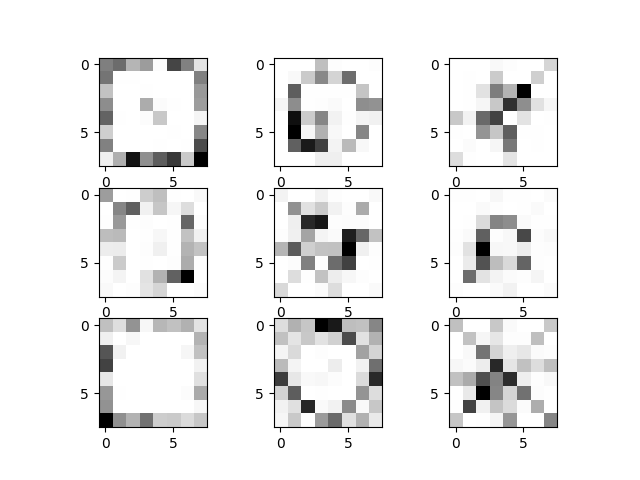
\includegraphics[width=1.0\linewidth]{lbcdi3.png}
    \caption{LB-CDI, $N_{train}=1000$}
    \label{fig: lbcdi_pattern}
    \end{subfigure}%
    \begin{subfigure}[t]{0.5\columnwidth}
    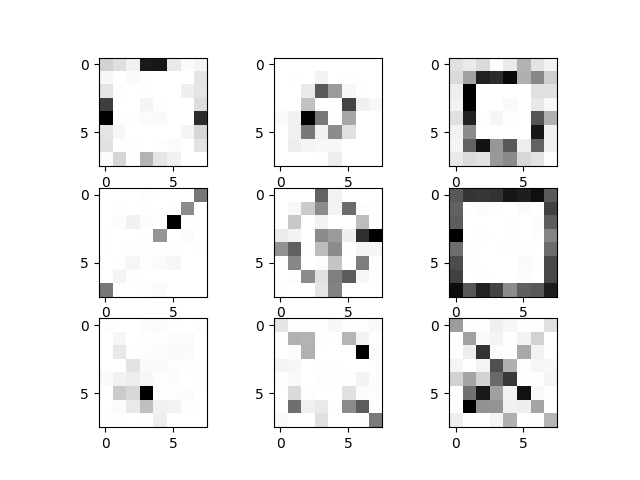
\includegraphics[width=1.0\linewidth]{svi_1000.png}
    \caption{SVI, $N_{train}=1000$}
    \label{fig: svi_pattern}
    \end{subfigure}
\caption{\small The recovered parameters after training with $1000$ data points using LB-CDI and SVI.}
\label{fig: pattern_nonamortized}
\end{figure}

Additionally, we did the parameter estimation experiments on \textsc{multi-mnist} dataset. And the experiment results are depicted in Fig. \ref{fig: parameter estimation multimnist}. Here, since the training set of \textsc{multi-mnist} is large, we did not do LB-CDI.

In Fig. \ref{fig: parameter estimation multimnist}, similar phenomenon has been observed. When we have large amount of training data, both AVI and ACP (Fig. \ref{fig: avi50000} and \ref{fig: ACP50000}) recovered parameters well. Even though AVI did not capture pattern $``1"$, it is indeed not trivial to separate pattern $``1"$ and $``7"$ in this dataset. However, SVI did not recover the parameters well. 

When we reduce the amount of training data, the number of patterns detected by AVI decreased largely, as three weight patterns are recovered as $``0"$, which also indicates worse latent representation learning.  However for ACP, although it messed up pattern $``4"$ and $``5"$, it recovered all other patterns, even with small amount of training data. 

\begin{figure*}
    \centering
    \begin{subfigure}[t]{0.2\textwidth}
        \centering
        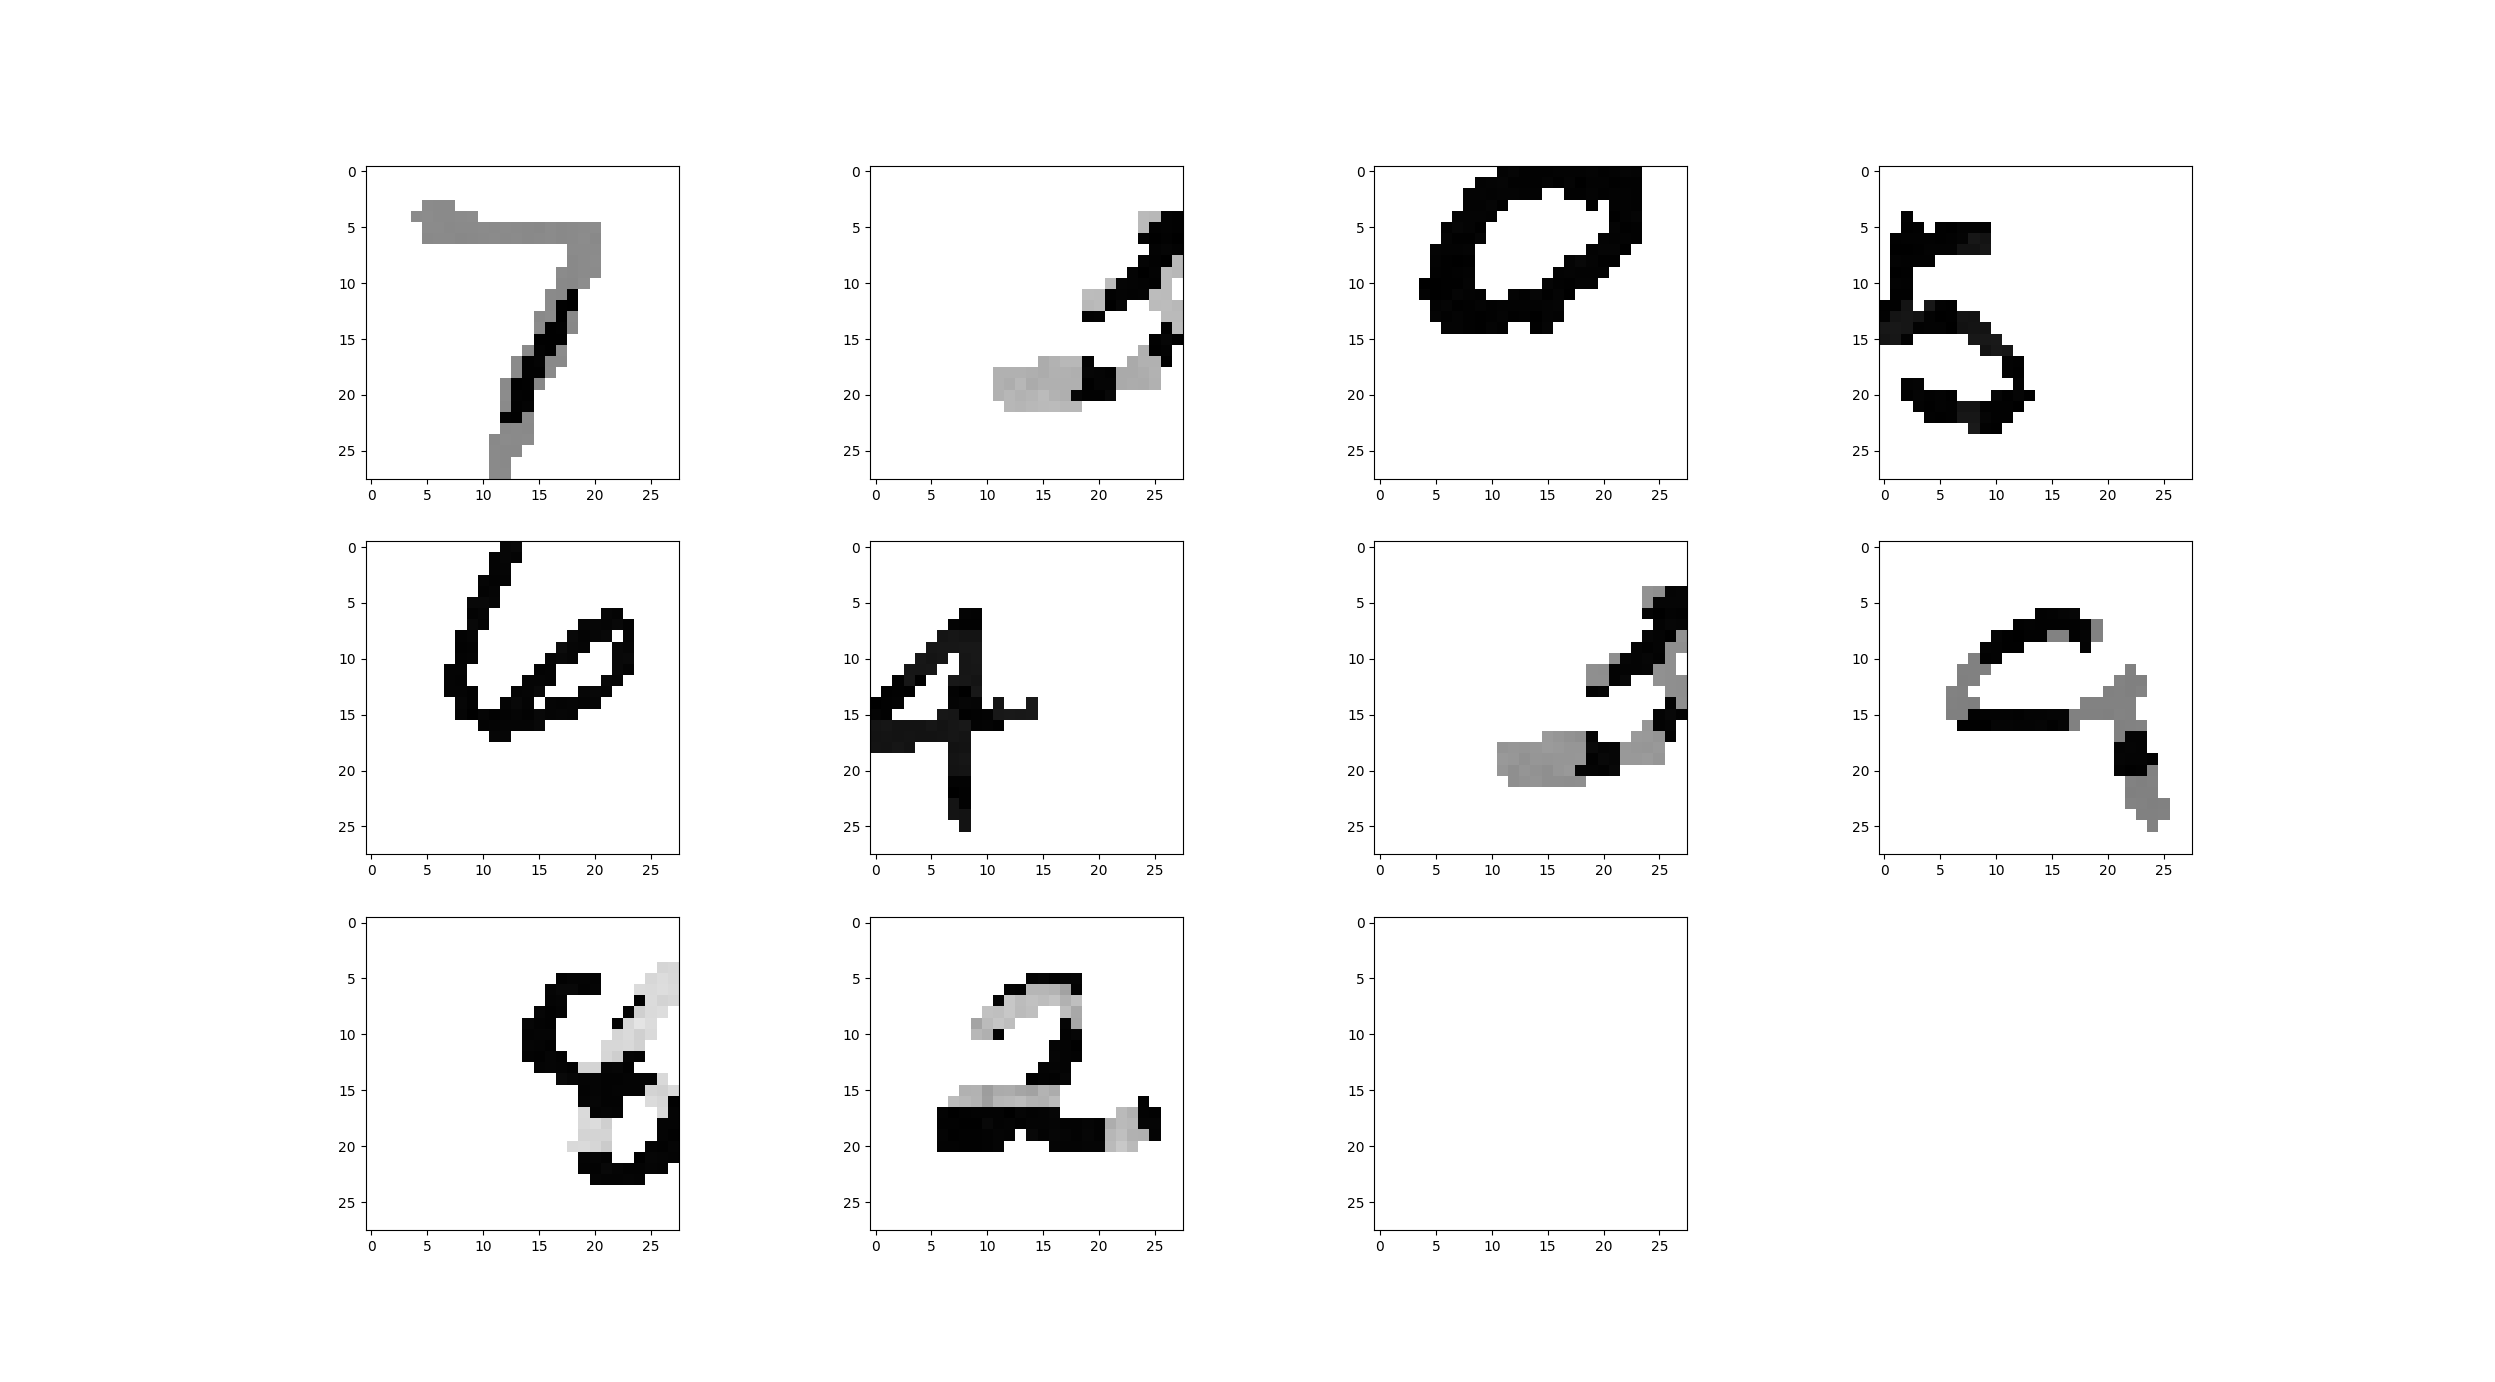
\includegraphics[width=1.0\linewidth]{avi2.png}
        \caption{AVI, $N_{train}=50K$}
        \label{fig: avi50000}
    \end{subfigure}%
    ~
    \begin{subfigure}[t]{0.2\textwidth}
        \centering
        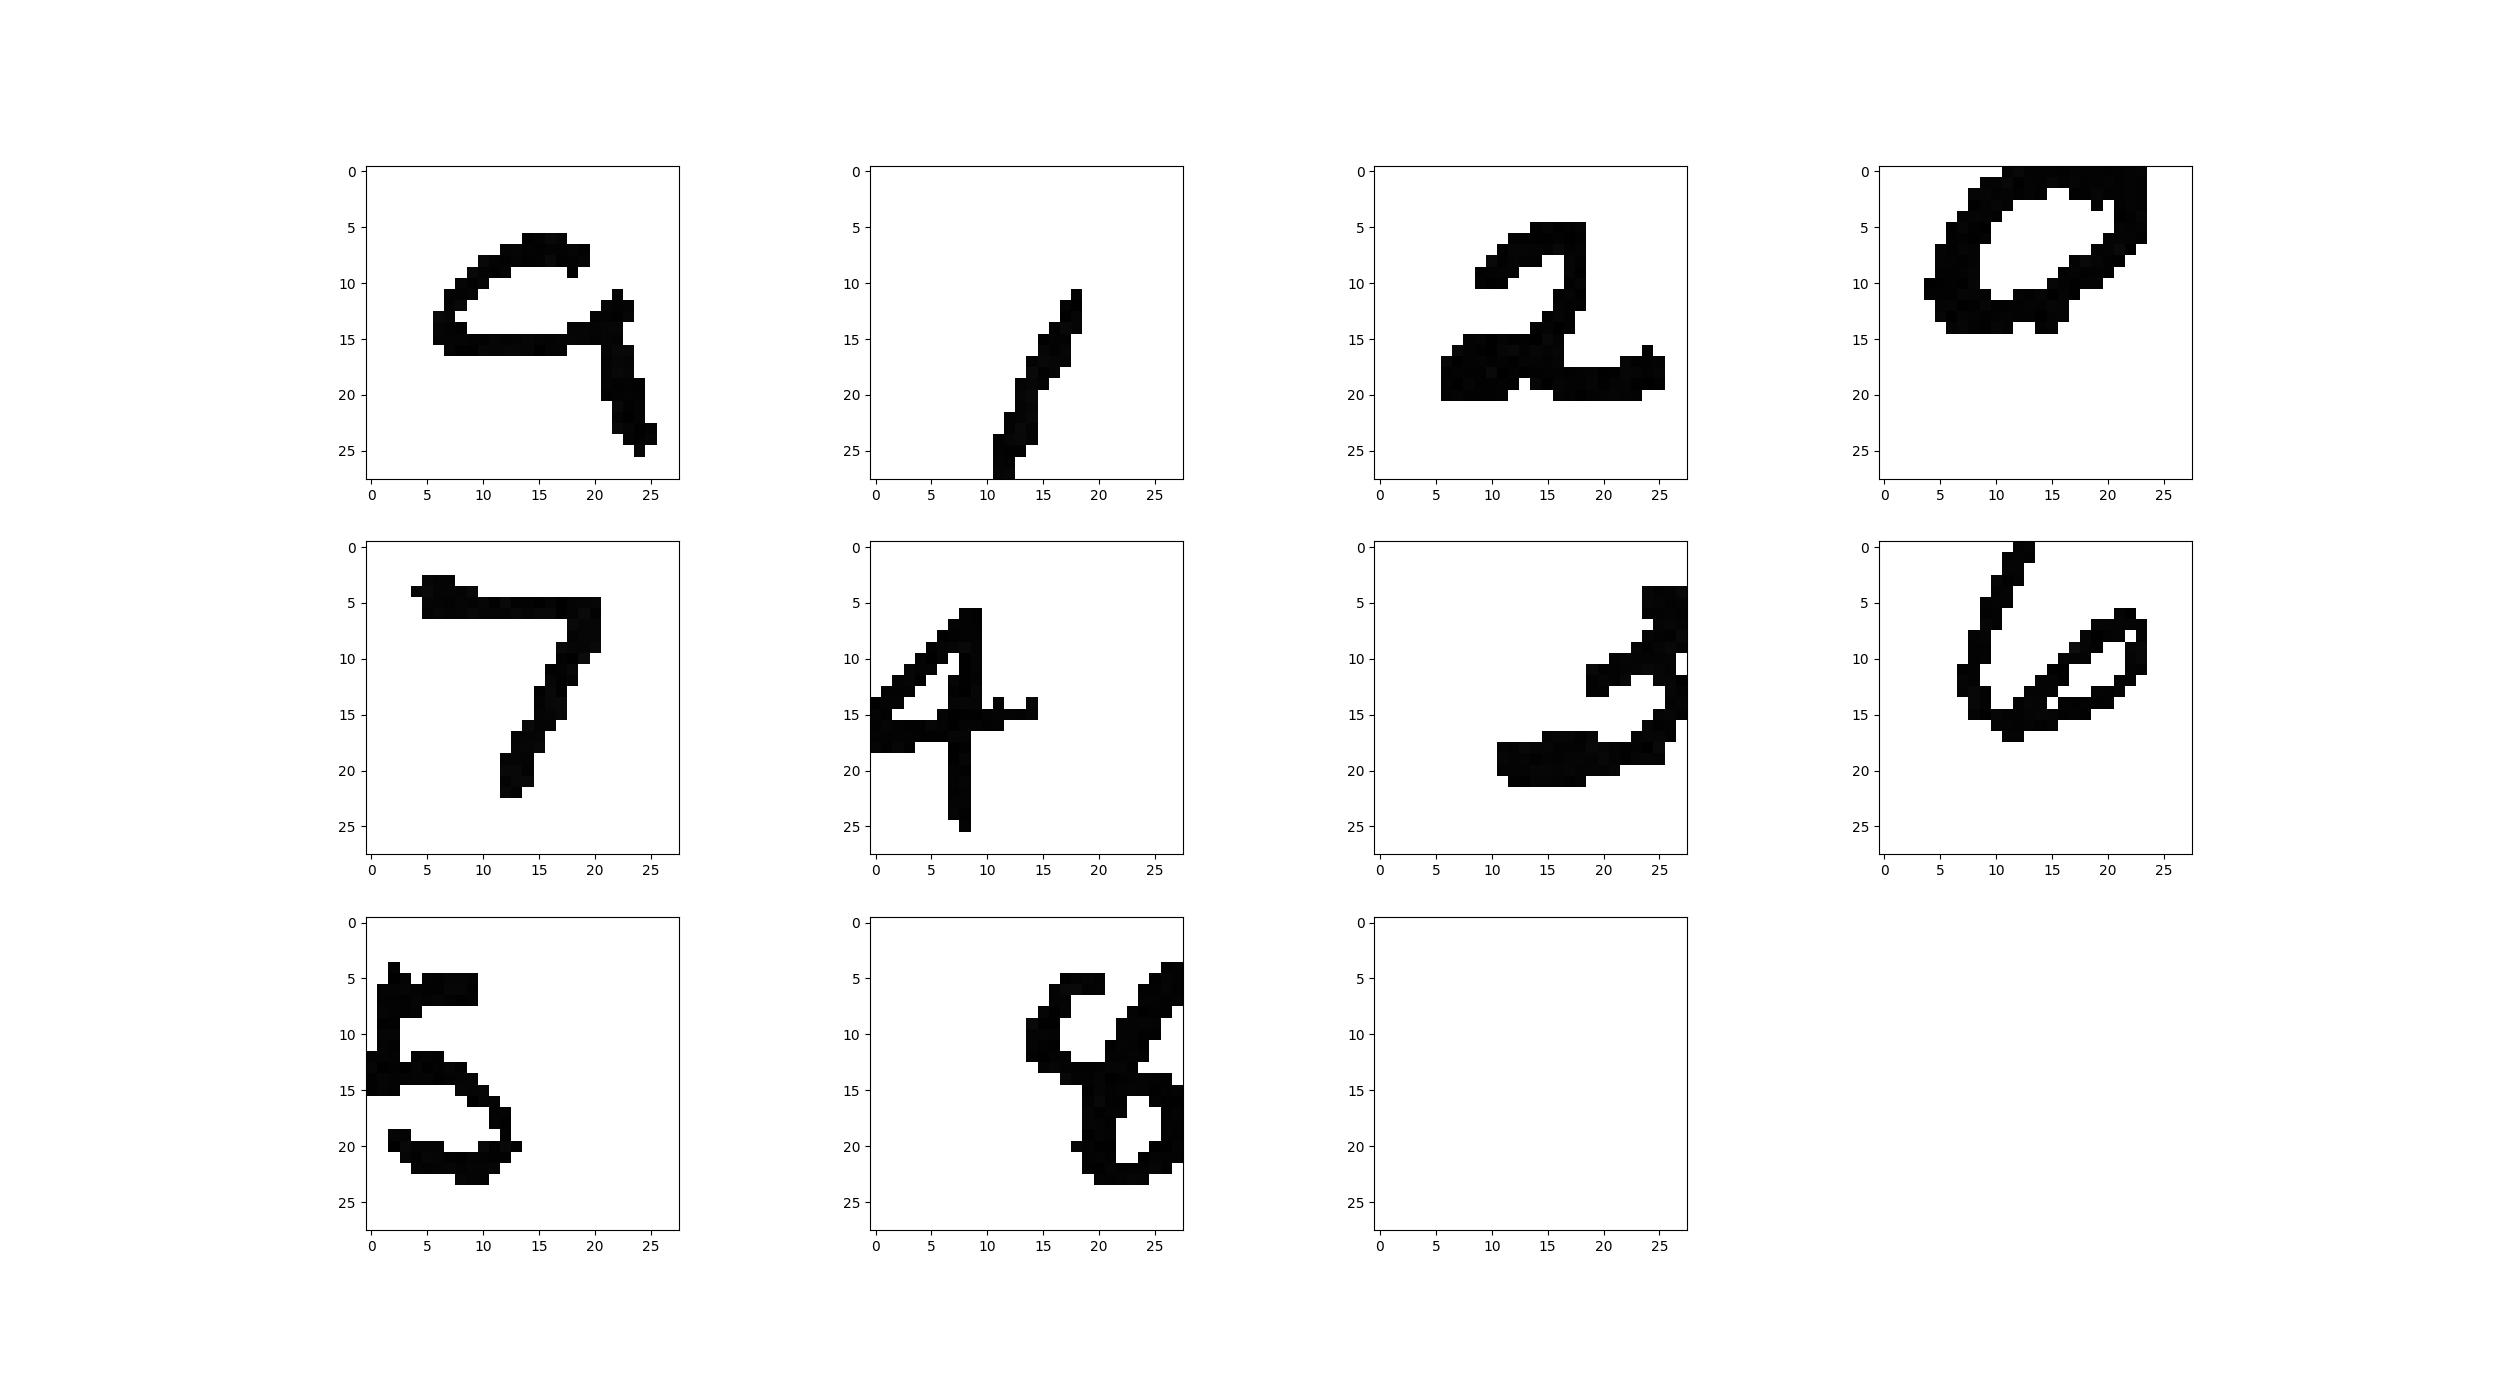
\includegraphics[width=1.0\linewidth]{ubacp50000.png}
        \caption{ACP, $N_{train}=50K$}
        \label{fig: ACP50000}
    \end{subfigure}%
    ~
    \begin{subfigure}[t]{0.2\textwidth}
        \centering
        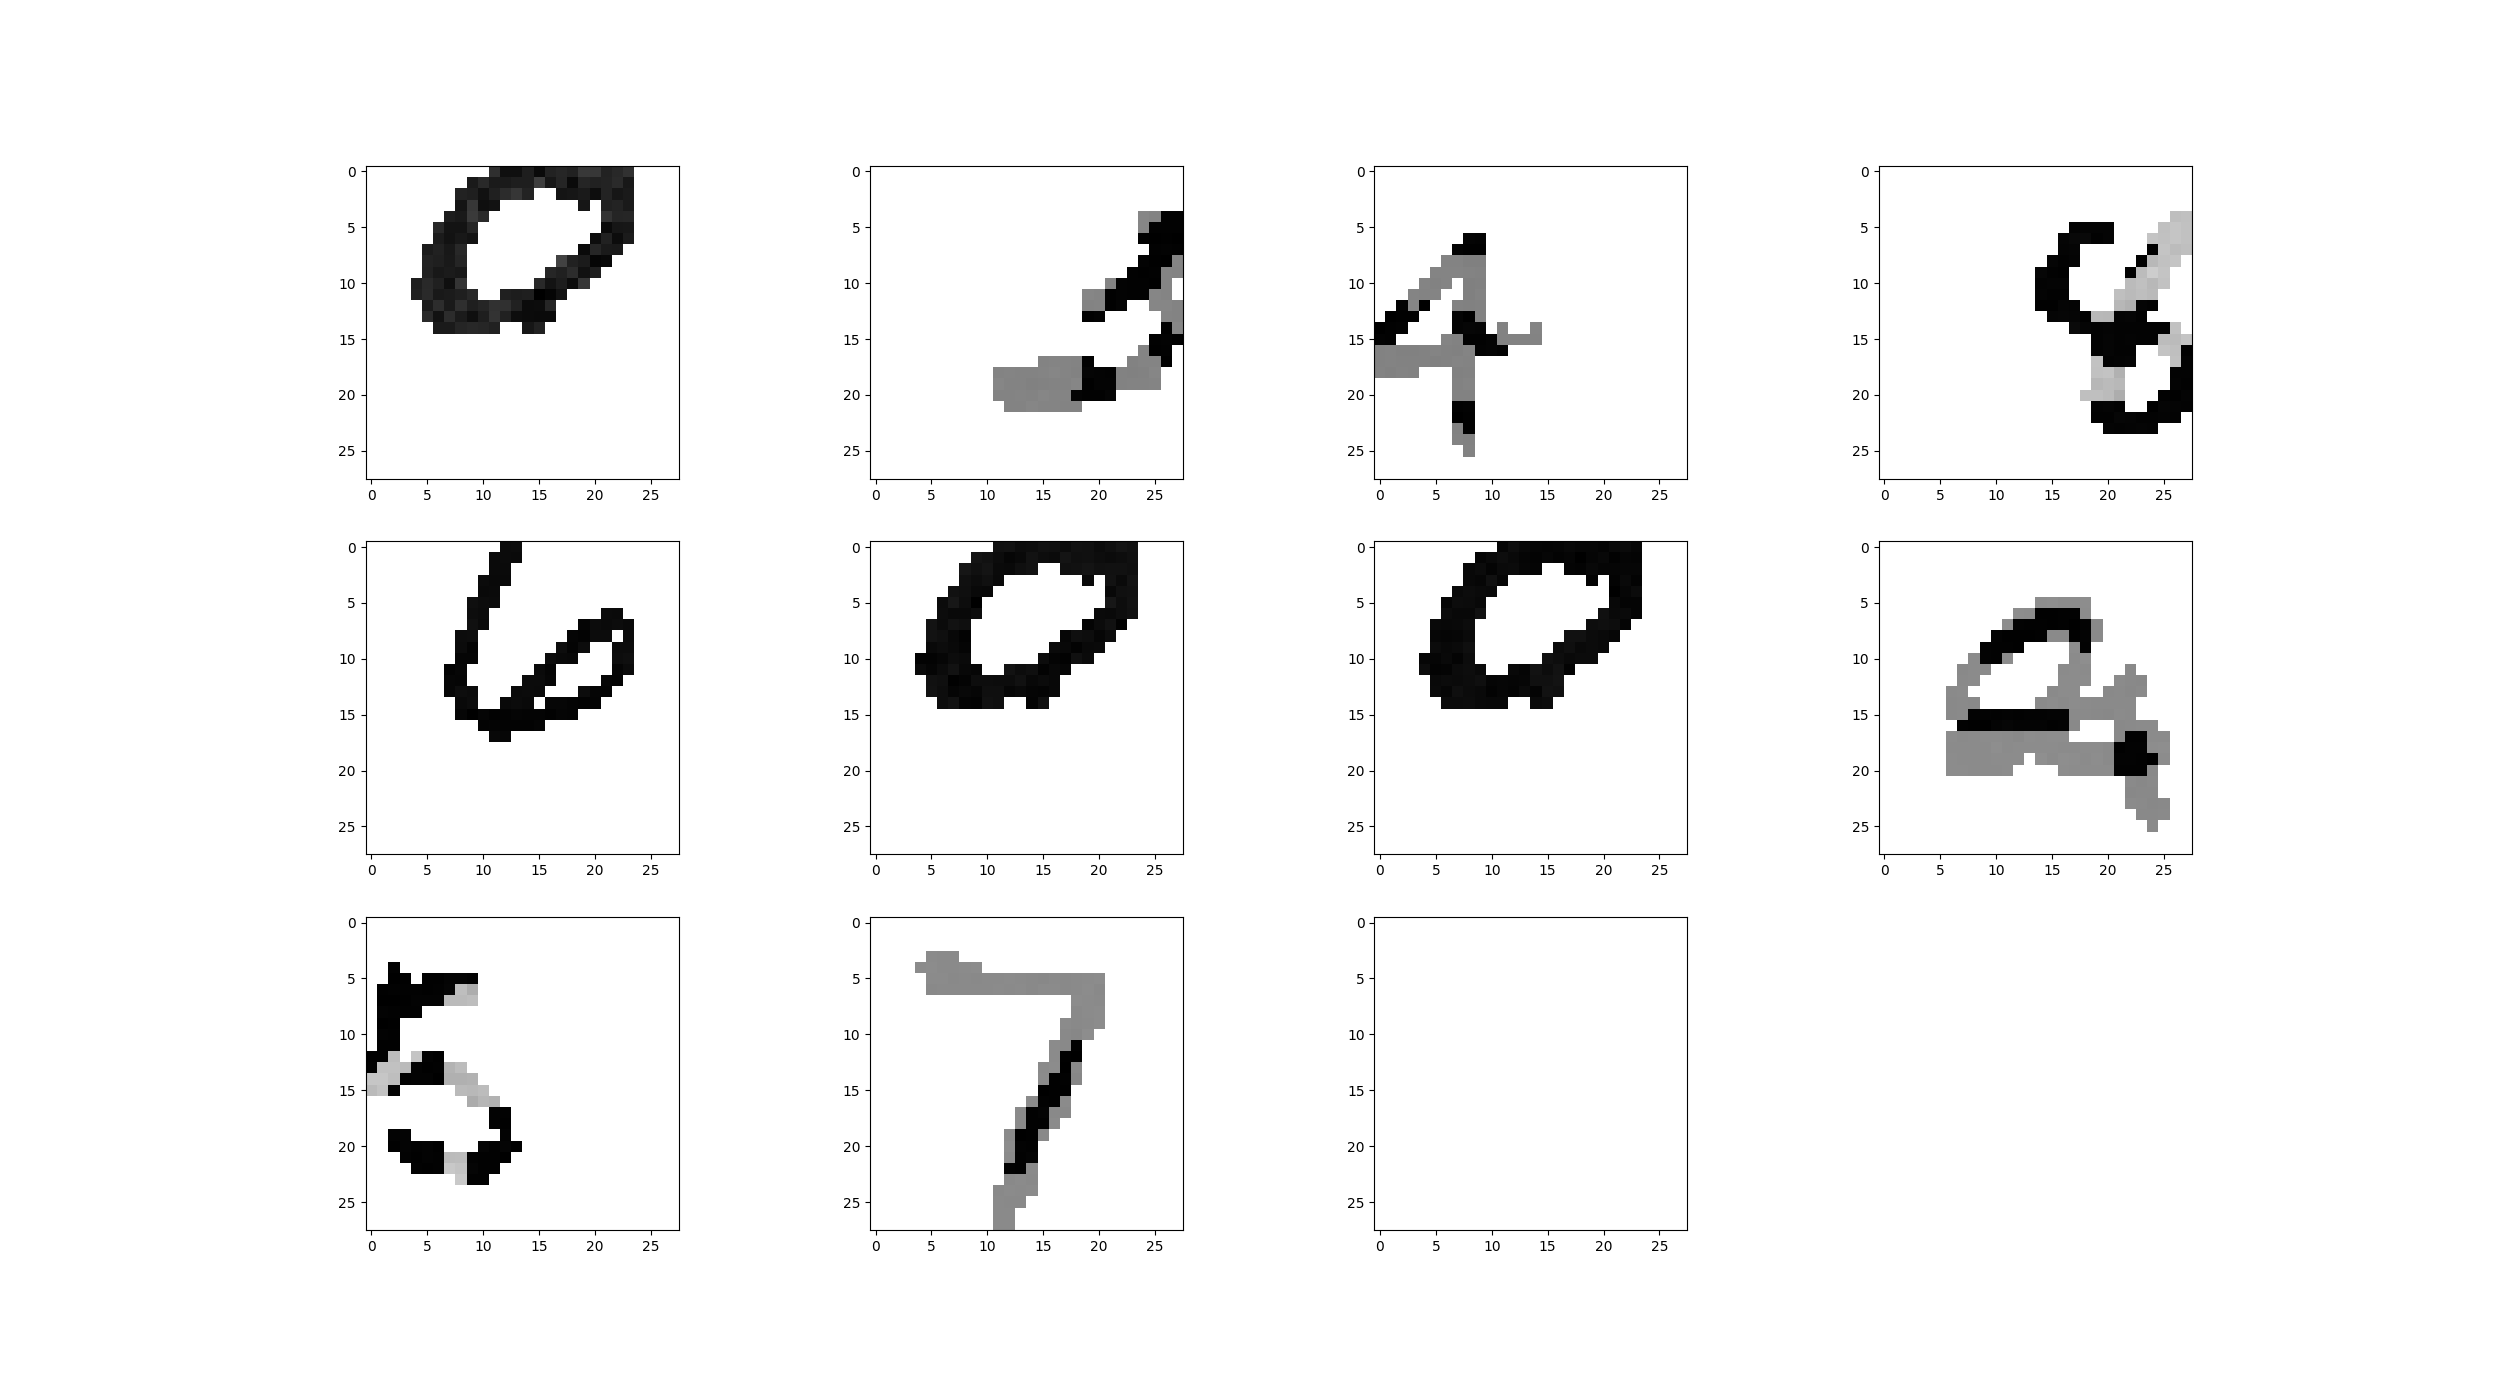
\includegraphics[width=1.0\linewidth]{avi_8000.png}
        \caption{AVI, $N_{train}=8K$}
        \label{fig: avi8000}
    \end{subfigure}%
    ~
    \begin{subfigure}[t]{0.2\textwidth}
        \centering
        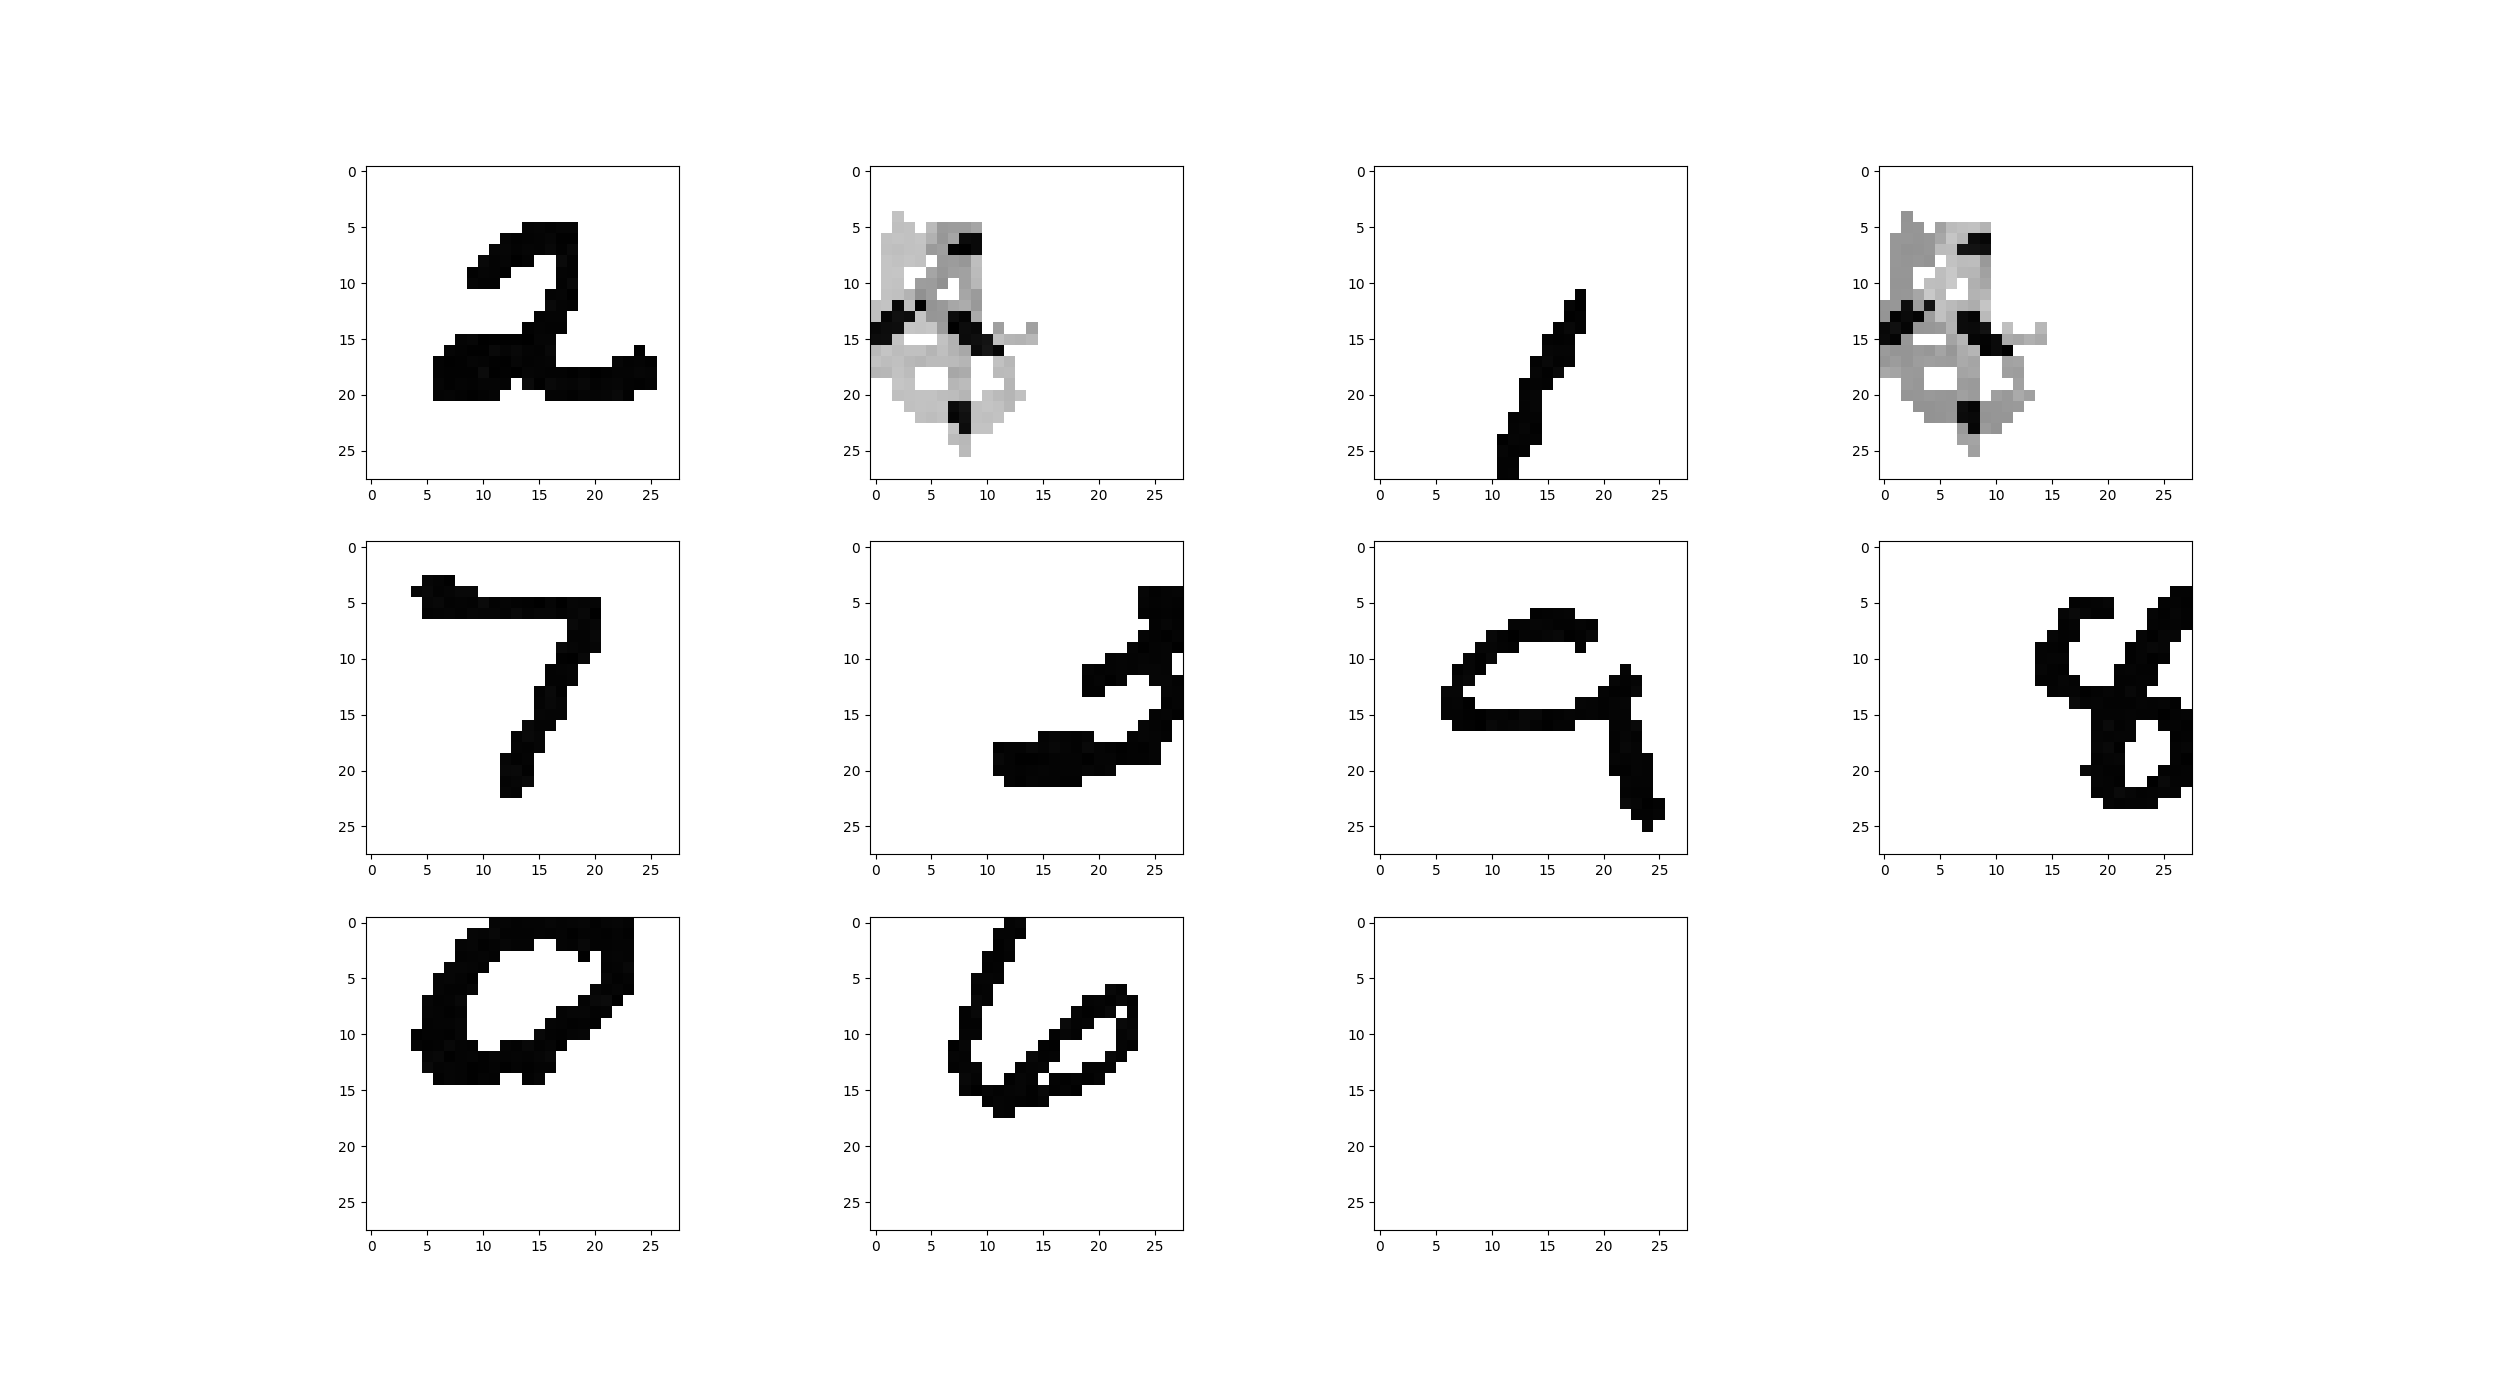
\includegraphics[width=1.0\linewidth]{ubacp_8000.png}
        \caption{ACP, $N_{train}=8K$}
        \label{fig: ACP8000}
    \end{subfigure}%
    \begin{subfigure}[t]{0.2\textwidth}
        \centering
        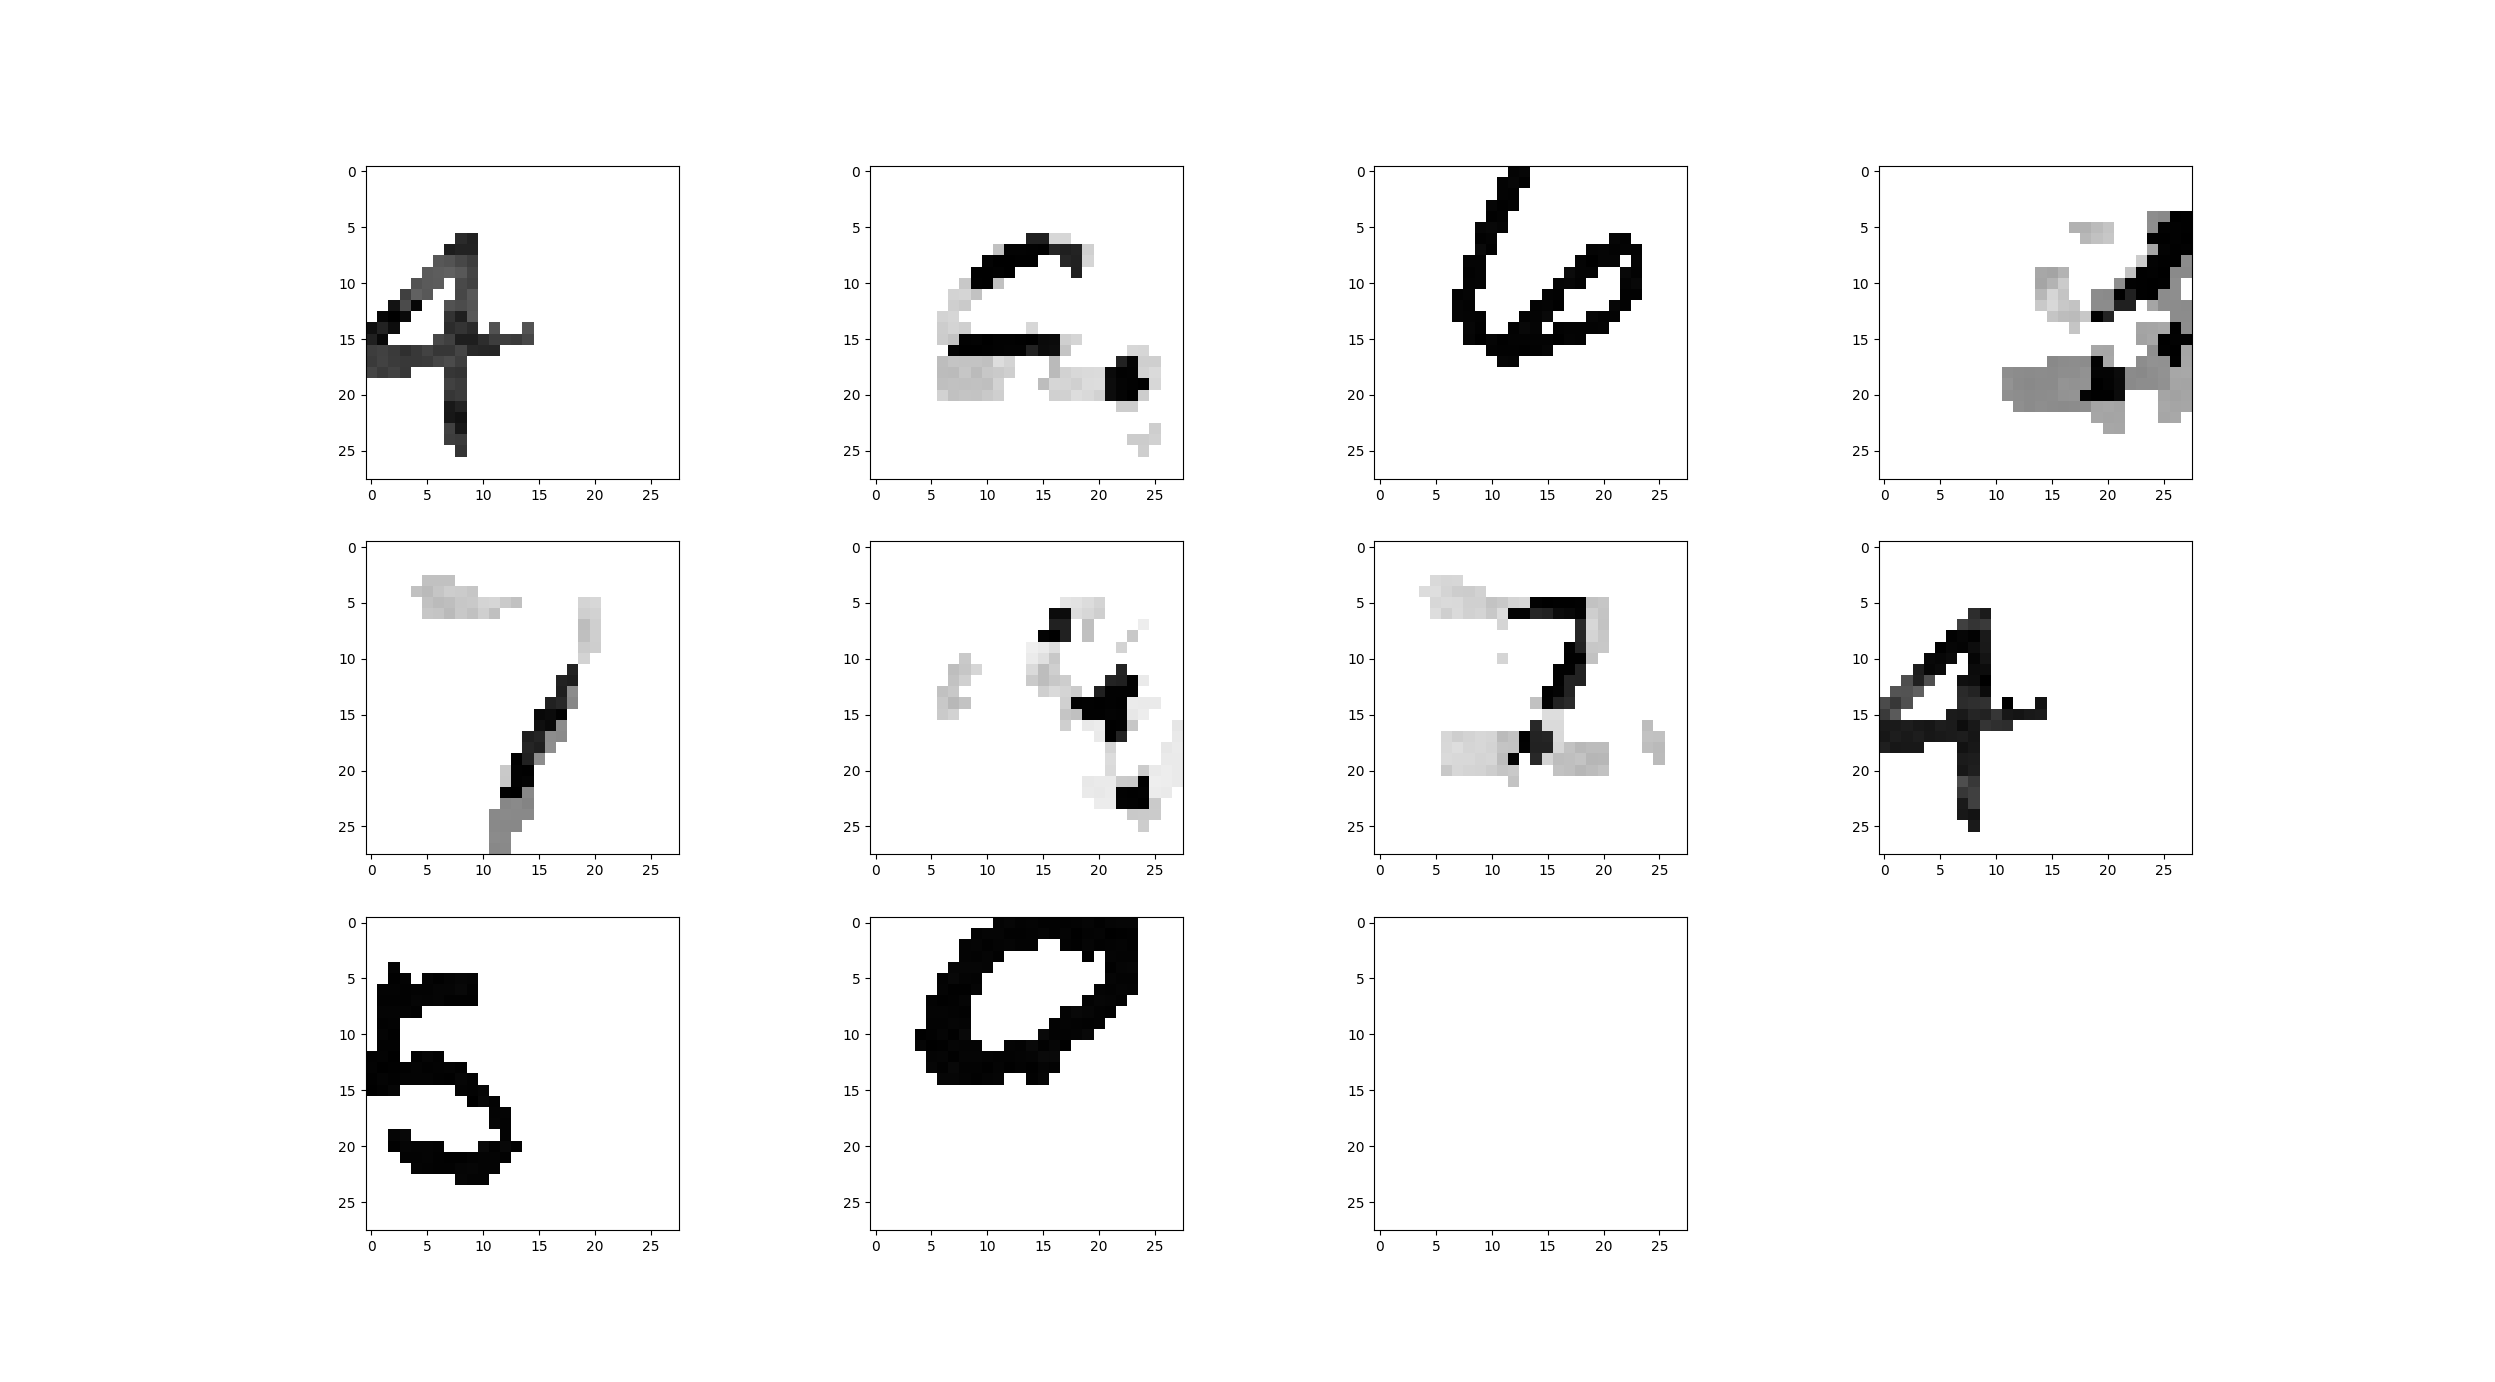
\includegraphics[width=1.0\linewidth]{svi50000.png}
        \caption{SVI, $N_{train}=50K$}
        \label{fig: svi50000}
    \end{subfigure}
\caption{\small The recovered parameters of \textsc{multi-mnist} after training with $50K$ and $8K$ data points using AVI, ACP and SVI.}
\label{fig: parameter estimation multimnist}
\end{figure*}

\section{Additional experiments}
\subsection{Document classification}
Herein, we aim to assess the impact of our inference method on \textsc{noisy-or} model's learned representations.
In particular, we rely on document classification task to evaluate the quality of the features learned by our model. 
%Here we rely on classification to assess the impact of our inference method on \textsc{noisy-or} model's learned representations.
%We conduct experiments on document classification task to exam the features learned by \textsc{noisy-or} model.
To this end, we use the Reuters corpus\footnote{https://www.nltk.org/book/ch02.html} from NLTK, which consists of $1.3$ million words and $10, 788$ news articles organized into $90$ categories. For this experiment, we retain the top $3$ categories,\footnote{the 3 classes containing the most documents.} namely \texttt{acq, earn} and \texttt{money-fx}. Each document is represented by its headline. 
We lemmatize the words, remove stop words, and remove words with less than $5$ occurrences. We obtain a final corpus of  $839$ unique words and $7030$ documents, including $5048$ for training and $1982$ for test. Similar to topic modeling, each document  is represented by a binary vector where each dimension indicates a word presence/absence. 
\begin{figure*}
    \centering
    %\vskip 0.2in
    \begin{subfigure}[t]{0.33\textwidth}
        \centering
        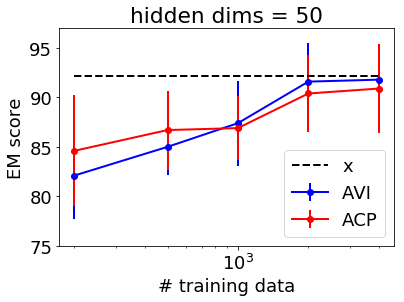
\includegraphics[width=1.0\linewidth]{reuters_cl_h50.png}
        \caption{}
        \label{fig: reuters_h50}
    \end{subfigure}%
    ~\begin{subfigure}[t]{0.33\textwidth}
        \centering
        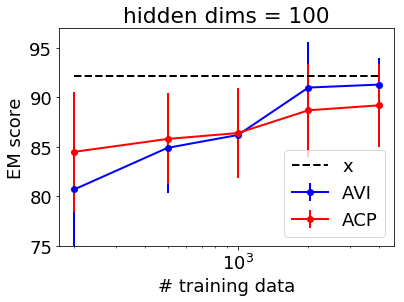
\includegraphics[width=1.0\linewidth]{reuters_cl_h100.png}
        \caption{}
        \label{fig: reuters_h100}
    \end{subfigure}%
    ~
    \begin{subfigure}[t]{0.33\textwidth}
        \centering
        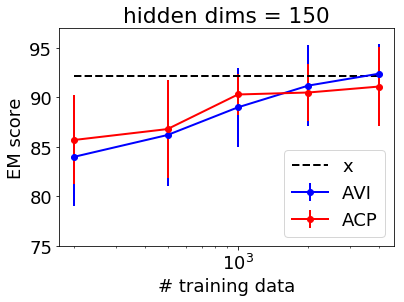
\includegraphics[width=1.0\linewidth]{reuters_cl_h150.png}
        \caption{}
        \label{fig: reuters_h150}
    \end{subfigure}
    
\caption{\small EM scores of AVI and ACP with different amount of training data and different hidden dimensions. The black dashed line indicates the classification performance with $\bx$ in test set as input.}
\label{fig: reuters_em}
\end{figure*}


After training AVI and ACP, we take the approximate posterior distribution $\big\{q(z_k^{(n)}=1|\bx^{(n); \bphi})\big\}_{k=1}^K$ as the latent representation of document $\bx^{(n)}$.
We evaluate the quality of learned representations on the test set. More specifically, we train a linear multilabel classifier, which takes the posterior distribution as input and predicts the document classes. We perform $5$-fold cross-validation and report the average EM scores. 

Fig.~\ref{fig: reuters_em} shows the classification performance with different amount of training data and different dimensionality of latent variables.  The black dashed line corresponds to the results obtained when performing classification on the original space $\bX$. 
We notice that when using  a training set of more than $1000$ documents, AVI achieves higher classification accuracy owing to its larger inference capacity and flexibility. However, its performance drops quickly as we reduce the size of the training set. In contrast, our ACP inference offers more stability w.r.t. to the amount of training examples, and reaches higher classification performance when using smaller training sets. 

We present in Fig. \ref{fig: reuters_hvis_50}, \ref{fig: reuters_hvis}  and \ref{fig: reuters_hvis_150} the t-SNE visualizations of the approximate posterior distributions learned by each model using 50, 100 and 150 hidden dimensions respectively. 
We observe that when using a small training set (middle and right columns), the \texttt{acq} and \texttt{money-fx} features learned by AVI tend to fuse together, while with ACP, we can still distinguish the three categories. 
This observation confirms our previous results and claims about the effectiveness of our model when lacking training data.

\begin{figure*}
    \centering
    \begin{subfigure}[t]{0.33\textwidth}
        \centering
        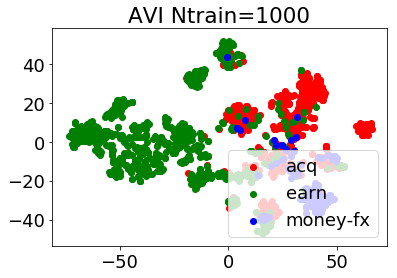
\includegraphics[width=1.0\linewidth]{reuters_avi1000_h50.png}
        \label{fig: reuters_h50_avi_1000}
    \end{subfigure}%
    ~
    \begin{subfigure}[t]{0.33\textwidth}
        \centering
        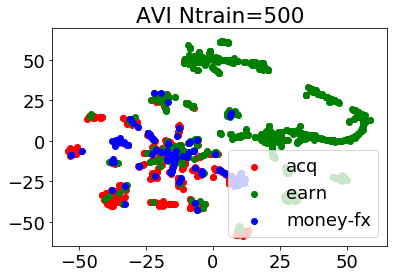
\includegraphics[width=1.0\linewidth]{reuters_avi500_h50.png}
        \label{fig: reuters_h50_avi_500}
    \end{subfigure}%
    ~
    \begin{subfigure}[t]{0.33\textwidth}
        \centering
        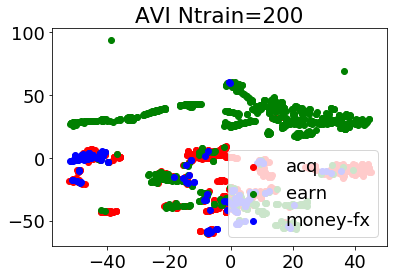
\includegraphics[width=1.0\linewidth]{reuters_avi200_h50.png}
        \label{fig: reuters_h50_avi_200}
    \end{subfigure}
    ~
    \begin{subfigure}[t]{0.33\textwidth}
        \centering
        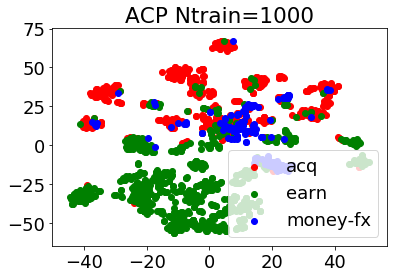
\includegraphics[width=1.0\linewidth]{reuters_acp1000_h50.png}
        \label{fig: reuters_h50_acp_1000}
    \end{subfigure}%
    ~
    \begin{subfigure}[t]{0.33\textwidth}
        \centering
        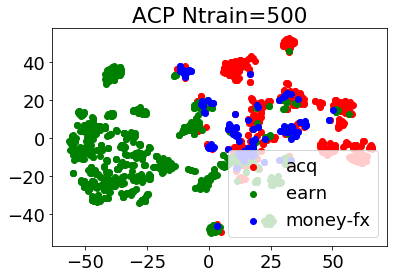
\includegraphics[width=1.0\linewidth]{reuters_acp500_h50.png}
        \label{fig: reuters_h50_acp_500}
    \end{subfigure}%
    ~
    \begin{subfigure}[t]{0.33\textwidth}
        \centering
        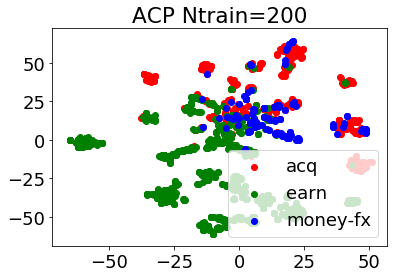
\includegraphics[width=1.0\linewidth]{reuters_acp200_h50.png}
        \label{fig: reuters_h50_acp_200}
    \end{subfigure}%
\caption{\small t-SNE visualization on latent representations on held out set when latent dimension is $50$.}
\label{fig: reuters_hvis_50}
\end{figure*}

\begin{figure*}
    \centering
    \begin{subfigure}[t]{0.33\textwidth}
        \centering
        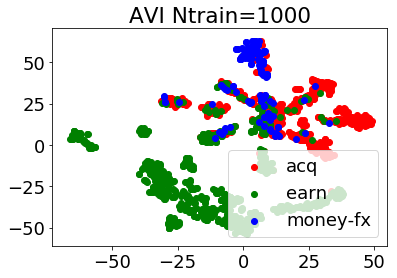
\includegraphics[width=1.0\linewidth]{reuters_avi1000.png}
        \label{fig: reuters_h100_avi_1000}
    \end{subfigure}%
    ~
    \begin{subfigure}[t]{0.33\textwidth}
        \centering
        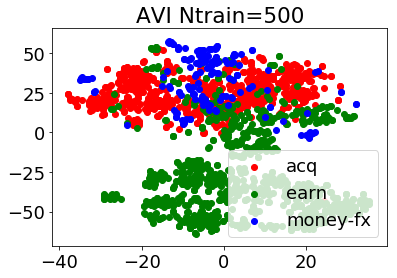
\includegraphics[width=1.0\linewidth]{reuters_avi500.png}
        \label{fig: reuters_h100_avi_500}
    \end{subfigure}%
    ~
    \begin{subfigure}[t]{0.33\textwidth}
        \centering
        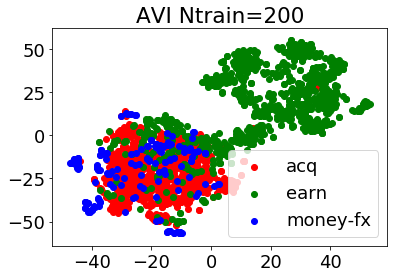
\includegraphics[width=1.0\linewidth]{reuters_avi200.png}
        \label{fig: reuters_h100_avi_200}
    \end{subfigure}
    ~
    \begin{subfigure}[t]{0.33\textwidth}
        \centering
        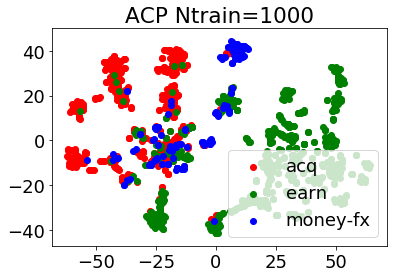
\includegraphics[width=1.0\linewidth]{reuters_acp1000.png}
        \label{fig: reuters_h100_acp_1000}
    \end{subfigure}%
    ~
    \begin{subfigure}[t]{0.33\textwidth}
        \centering
        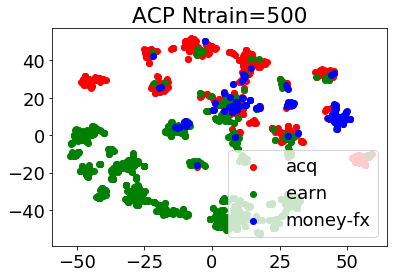
\includegraphics[width=1.0\linewidth]{reuters_acp500.png}
        \label{fig: reuters_h100_acp_500}
    \end{subfigure}%
    ~
    \begin{subfigure}[t]{0.33\textwidth}
        \centering
        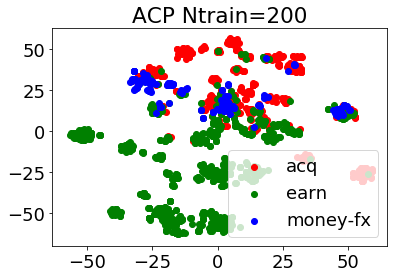
\includegraphics[width=1.0\linewidth]{reuters_acp200.png}
        \label{fig: reuters_h100_acp_200}
    \end{subfigure}%
\caption{\small t-SNE visualization on latent representations on held out set when latent dimension is $100$.}
\label{fig: reuters_hvis}
\end{figure*}

\begin{figure*}
    \centering
    \begin{subfigure}[t]{0.33\textwidth}
        \centering
        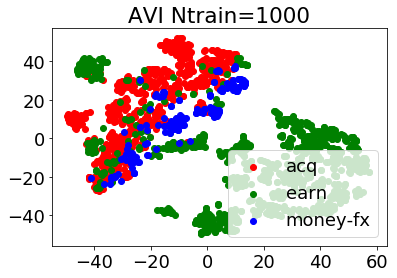
\includegraphics[width=1.0\linewidth]{reuters_avi1000_h150.png}
        \label{fig: reuters_h150_avi_1000}
    \end{subfigure}%
    ~
    \begin{subfigure}[t]{0.33\textwidth}
        \centering
        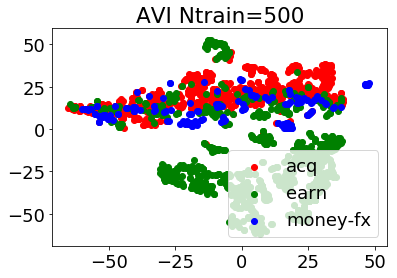
\includegraphics[width=1.0\linewidth]{reuters_avi500_h150.png}
        \label{fig: reuters_h150_avi_500}
    \end{subfigure}%
    ~
    \begin{subfigure}[t]{0.33\textwidth}
        \centering
        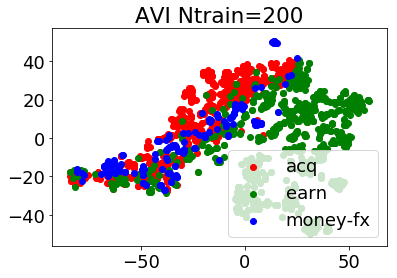
\includegraphics[width=1.0\linewidth]{reuters_avi200_h150.png}
        \label{fig: reuters_h150_avi_200}
    \end{subfigure}
    ~
    \begin{subfigure}[t]{0.33\textwidth}
        \centering
        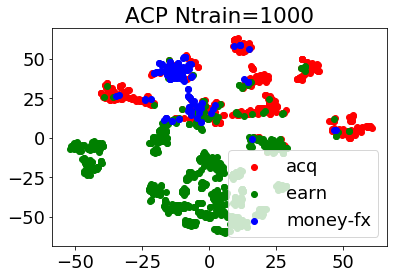
\includegraphics[width=1.0\linewidth]{reuters_acp1000_h150.png}
        \label{fig: reuters_h150_acp_1000}
    \end{subfigure}%
    ~
    \begin{subfigure}[t]{0.33\textwidth}
        \centering
        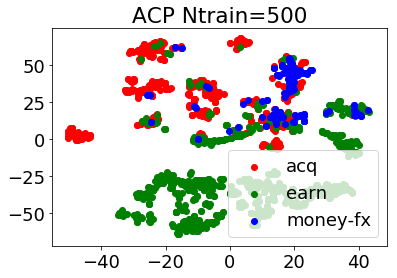
\includegraphics[width=1.0\linewidth]{reuters_acp500_h150.png}
        \label{fig: reuters_h150_acp_500}
    \end{subfigure}%
    ~
    \begin{subfigure}[t]{0.33\textwidth}
        \centering
        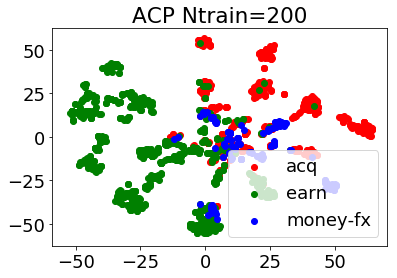
\includegraphics[width=1.0\linewidth]{reuters_acp200_h150.png}
        \label{fig: reuters_h150_acp_200}
    \end{subfigure}
\caption{\small t-SNE visualization on latent representations on held out set when latent dimension is $150$.}
\label{fig: reuters_hvis_150}
\end{figure*}

%\subsection{Collaborative filtering}
%\todo{Todo: still working on this subsection}
%Here, we perform collaborative filtering on \textsc{noisy-or} model with AVI and ACP inference. We conduct experiments on MovieLens 100K dataset, which is a stable benchmark contains 100,000 ratings from 1000 users on 1700 movies. We form our dataset $\bX$ as the following: if user $n$ rates movie $i$ as $5$, then $x_{ni}=1$, otherwise $x_{ni}=0$. We split our dataset to training and test set. For training set, we include all the observed data, while for test set we randomly remove one movie $x_i$ rated as $5$ per user. As suggested in~\cite{blei2003latent}, we evaluate the performance of collaborative filtering by the predictive perplexity, which is defined as
%\begin{align}
%    predictive-perplexity=\exp\bigg(-\frac{1}{N}\sum_{n=1}^N \logp(x_i^{(n)}=1|\bx^{(n)}_{-i})\bigg)
%\end{align}


%\subsection{Optimizing upperbound*}
%In ELBO (eq. \ref{eq: elbo for nor}), the expected log likelihood for positive points still requires sampling from posterior. Here we perform experiment to avoid sampling by replacing the positive likelihood with its upperbound. Now the objective function becomes
%\begin{align}
%    \mathcal{L(\bx; \btheta, \bphi)} & = \sum_{i:x_i=1}^D\mathbb{E}_{\qphi(\bz|\bx)}[\log \tilde{p}_{\btheta}(x_i=1|\bz, \bphi)] 
%     + \sum_{i:x_i=0}^D \mathbb{E}_{\qphi(\bz|\bx)}[\log p(x_i=0|\bz)] \nonumber\\
%    & - D_{KL}\Big(\pqx||\ppz\Big) \leq \log p_{\btheta}(\bx)
%\label{eq: upllh for nor}
%\end{align}
%which has tractable computation without Monte Carlo sampling. 
%\begin{figure}[ht]
%\centering
%    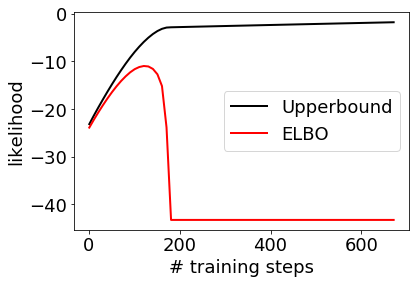
\includegraphics[width=0.4\linewidth]{optimize_ub.png}
%    \caption{\small Learning curves for optimizing upperbound of ELBO}
%    \label{fig: ubllh}
%\end{figure}

%As shown in Fig. \ref{fig: ubllh}, when we maximize the ELBO upperbound, the upperbound becomes more and more loose. The ELBO firstly increases and then drops quickly and converges with a bad likelihood. 




%\subsection{Weight ACP*}
%Inspired by eq.~(\ref{eq: factorizedPosterior}), we experiment the other form of approximate posterior as 
%\begin{align}
%    q(z_k=1 |\bx, \bpsi, \blambda) = 
%    \sigma\left(\sum_{i:x_i=1}\psi_i\theta_{ik} - \sum_{i:x_i=0}\lambda_i\theta_{ik} + \log \frac{\mu_k}{1-\mu_k}\right).
%\label{eq:factorizedposterior2}
%\end{align}
%Here, $\lambda_i$ is also the output of a neural network. And $\blambda$ and $\bpsi$ are constrained to be positive. We name the new approach as weighted-ACP. As shown in Fig. \ref{fig: weightvpn} and Fig. \ref{fig: weightvpn_reuters}, for both density estimation and latent representation learning tasks, weighted-ACP achieves similar performance comparing with ACP with more parameters to train. Hence we do not consider weighted-ACP in our experiments.
%\begin{figure}[ht]
%\centering
%    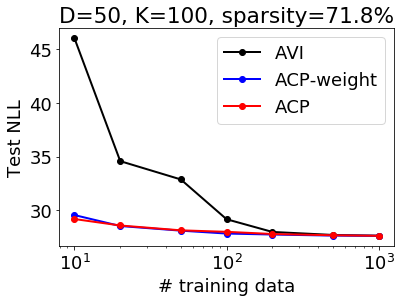
\includegraphics[width=0.4\linewidth]{weight_vpn_100_50_dense.png}
%    \caption{\small Negative ELBO on Toy-Sample dataset with different number of training data}
%    \label{fig: weightvpn}
%\end{figure}
%\begin{figure}[ht]
%\centering
%    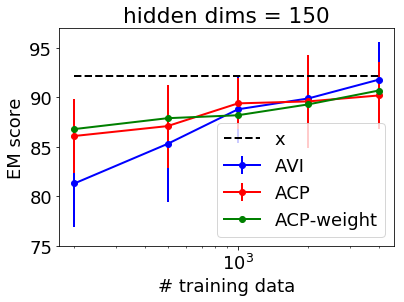
\includegraphics[width=0.4\linewidth]{weight_vpn_reuters_h150.png}
%    \caption{\small Document classification performance on Reuters dataset}
%    \label{fig: weightvpn_reuters}
%\end{figure}
%
%


\pagebreak

\bibliography{example_paper} 
\bibliographystyle{ieeetr}
\end{document}